\documentclass[a4paper,12pt]{article}

\usepackage{geometry}
\geometry{margin=1in}

\usepackage[english]{babel}
\usepackage{authblk}
\usepackage{geometry}
\usepackage{graphicx}
\usepackage{amsmath}
\usepackage{amssymb}
\usepackage{amsthm}
\usepackage{mathrsfs}
%\usepackage[colorlinks,bookmarksopen,bookmarksnumbered,citecolor=red,urlcolor=red]{hyperref}
\usepackage{apalike}
\usepackage[utf8x]{inputenc}
%\usepackage{nameref,hyperref}
% line numbers
%\usepackage[right]{lineno}
% ligatures disabled
\usepackage{microtype}
\usepackage{multirow}
\usepackage[table]{xcolor}
\definecolor{lightgray}{HTML}{e6e6e6}

\usepackage{tikz}
\usetikzlibrary{arrows}
\usetikzlibrary{shapes, positioning, calc}

\usepackage{float}

%\DisableLigatures[f]{encoding = *, family = * }
% color can be used to apply background shading to table cells only
\usepackage[table]{xcolor}
% array package and thick rules for tables
\usepackage{array}
% create "+" rule type for thick vertical lines
\newcolumntype{+}{!{\vrule width 2pt}}

\usepackage{setspace}
\doublespacing

\newcommand{\RR}{\mathbb{R}}
\DeclareMathOperator*{\V}{V}
\DeclareMathOperator*{\argmax}{argmax}
\newcommand{\R}[1]{\texttt{#1}}
\newcommand{\acos}{\text{arccos}}


\newcommand{\hl}[1]{\textcolor{magenta}{#1}}
\renewcommand{\baselinestretch}{2}






\newcommand\BibTeX{{\rmfamily B\kern-.05em \textsc{i\kern-.025em b}\kern-.08em
T\kern-.1667em\lower.7ex\hbox{E}\kern-.125emX}}

\def\volumeyear{2018}

\begin{document}

%\runninghead{PCADSC}

\title{Exploratory data structure comparisons: Three new visual tools based on Principal Component Analysis}

\author[1]{}
%\author[1]{Anne Helby Petersen}
%\author[1]{Bo Markussen}
%\author[3]{Karl Bang Christensen}
%\affil[1]{Department of Public Health, University of Copenhagen, Copenhagen, Denmark}
%\affil[2]{Department of Mathematical Sciences, University of Copenhagen, Copenhagen, Denmark}
\date{}
\maketitle


%\corrauth{Anne Helby Petersen}
%\email{ahpe@sund.ku.dk}

\renewcommand{\abstractname}{Abstract}
\renewcommand{\figurename}{Figure}
\renewcommand{\tablename}{Table}

\begin{abstract}
Datasets are sometimes divided into distinct subsets, e.g. due to multi-center sampling, or to variations in instruments, questionnaire item ordering or mode of administration, and the data analyst then needs to assess whether a joint analysis is meaningful. The Principal Component Analysis-based Data Structure Comparisons (PCADSC) tools are three new non-parametric, visual diagnostic tools for investigating differences in structure for two subsets of a dataset through covariance matrix comparisons by use of principal component analysis. The PCADCS tools are demonstrated in a data example using European Social Survey data on psychological well-being in three countries, Denmark, Sweden, and Bulgaria. The data structures are found to be different in Denmark and Bulgaria, and thus a comparison of for example mean psychological well-being scores is not meaningful. However, when comparing Denmark and Sweden, very similar data structures, and thus comparable concepts of well-being, are found. Therefore, inter-country comparisons are warranted for these countries.
\end{abstract}






%% Include all macros below


\section*{Introduction}\label{sec:introduction}


Data comparability is a classical topic in statistics and a recurring one in psychometrics. Often, psychometric data will be collected in such a way that it is essentially divided into several subsets whose comparability needs to be assessed empirically. This happens for instance when data are collected across several centers (or countries) or when different versions of an instrument, the mode of administration, or the order of survey questionnaire items are applied. While a mixture of modes of administration, for example mail and telephone, can improve response rates in surveys, it can also be quite problematic by inducing differences in response behavior that may lead to biased results \cite{Brambilla1987,McHorney1994}. Powers, Mishra, and Young report effects of mode of administration on changes in mental health scores that are of a magnitude that is considered to be clinically meaningful \cite{Powers2005}, so the comparability issue is not just a statistical puzzle. Similarly, combining data obtained from different sampling schemes can also be problematic, as illustrated by Liu (2016), who warns against combining online panel data with intercept samples (a pool of respondents obtained through banners, ads, or promotions).\nocite{Liu2016} But mixing several data collection methods is an essential part of the psychometric methodology, as it allows us to simultaneously build on existing methods and answer new, empirical questions. However, if we do not address the question of comparability among the data subsets arriving from e.g. different countries, we risk conducting analyses whose most fundamental assumptions are not satisfied.

The comparability issue in these examples can be summarized as follows: Assume that we have two datasets with the same variables, but different observations, often represented as a single dataset with a subset-inducing variable, and that we wish to compare them without specifying a model, or even a variable of interest. The central question is then whether the two datasets can readily be combined for the purpose of later data analysis, or if the subset-inducing variable implies heterogeneity that must be dealt with in later statistical modelling.

Sophisticated methods for addressing this question are available when we are willing to assume a statistical model. But this places the effort of assessing data comparability very late in the data analysis process and it makes the comparability assessment ad-hoc, as it essentially relies on the appropriateness of the modeling choices, which again depends on the structure of the data. The use of (parametric) models does thus not constitute a general data structure comparison method, but rather a fitted-model comparison method. It addresses the interplay between the model and the data, not the data alone. However, useful tools for initial, exploratory investigations of data comparability %that help researchers identify potential problems or challenges early in the study design development 
are mostly absent. What is needed are procedures that compare differences in data structures in two subsets of a dataset without assuming neither directional nor hierarchical relationships between the variables.  Simple methods like variable-by-variable tests of distributional differences suffer from the drawback that they only address marginal differences and ignore the interplay between variables, but entry-by-entry comparisons of two empirical correlation matrices quickly become unmanageable as the number of variables increase.

%While the issue is not in any way new, its relative importance is increasing due to new developments in data availability and data collection. Classical statistical methods are generally aimed at analyzing data from designed experiments and historically, statistical analyses have been conducted by researchers who knew the design and the source of the dataset well. However, the origin stories of datasets have changed over time and today, a lot of data are accumulated without a specific purpose in mind, as data collection and sharing has become easier and more affordable through the development of new technologies. This new era of data sharing facilitates a tremendous amount of new research, as data on all sorts of topics are now readily available online for everyone to use. However, large scale publicly available datasets, such as the PISA (Programme for International Student Assessment) data and European Social Survey (ESS) data, are often used by data analysts that are far removed from the data producers and therefore, problem-specific recommendations about e.g. potential instrument-induced challenges in the datasets may not be available for these data analysts. For this reason, a thorough investigation of data structure comparability becomes a crucial step in any meaningful data analysis when using such open-source data.


We propose three visual tools for data structure comparisons, which we will refer to collectively as Principal Component Analysis-based Data Structure Comparisons (PCADSC). These methods use principal component decomposition of the empirical covariance matrix in the two subsets to create intuitive visualizations of data structure differences. The use of PCA implies that we can only compare datasets with numerical variables and that we focus on the linear aspect of the  data structures. The proposed tools are implemented in the \texttt{R} package \texttt{PCADSC} \cite{PCADSC}. Below, we describe the procedures and present a worked data example using open source, online available data on psychological well-being in three European countries from the European Social Survey. More specifically, we compare data from Denmark with data from Bulgaria and Sweden, respectively, to investigate whether or not data on psychological well-being can be combined across countries - a question that is ignored e.g. when international rankings of happiness among countries are posted by the UN \textit{World Happiness Report} project \cite{WHR2016}.


\section*{PCA-based tools for data structure comparisons}\label{sec:pcadscintro}


PCADSC compares the covariance matrices of two subsets of a dataset. If all variables in the subsets are jointly normal with known means, the covariance matrices are sufficient statistics describing the joint distribution of all the variables, but even without the normality assumption, pairwise correlations and marginal variable variances are still interesting quantities describing linear interrelations between variables. This makes the empirical covariance matrix a reasonable place to start looking for differences in data structures. Computing empirical covariance matrices for the two subsets and comparing them entry-by-entry becomes increasingly difficult as the number of variables increases and for this reason we decompose and recompose the covariance matrices using \textit{principal component analysis} (PCA) to get an overview of differences between the two subsets. We refer to Appendix S1 for a brief introduction to PCA. 

We assume that the variables have been standardized before PCA is conducted, which is equivalent to working with the empirical correlation matrices rather than the empirical covariance matrices. We also assume that all considered variables have a numerical interpretation, for example by being continuous or ordinally categorical. Moreover, we use the following notation: 
$\mathbf{X} \in \RR^{n_x \times d} $ and $\mathbf{Y} \in \RR^{n_y \times d} $ are datasets containing the same number of variables, $d$, but possibly different numbers of observations, $n_x$ and $n_y$. We use $X_j$ to refer to the $j$th variables of $\mathbf{X}$ and $x_{ij}$ to refer to the $i$th observation  within that variable, while $x_{i \cdot}$ is the full $i$th observation row. Note that $X_j \in \RR^{n_x}$, $x_{ij} \in \RR$, and $x_{i \cdot} \in \RR^d$. We let $\bar{X} = (\bar{X}_1, ... , \bar{X}_d)^T = \frac{1}{n_x} \sum_{i = 1} x_{i \cdot}$ denote the variable averages and use $S_x =  \frac{1}{n_x - 1} \sum_{i = i}^n (x_{i \cdot} - \bar{X}) - (x_{i \cdot} - \bar{X})^T \in \RR^{d \times d}$ to denote the empirical covariance matrix of $\mathbf{X}$. 



\subsection*{Using PCA for data structure comparisons}
%PCA qualifies as an appealing first step in structural comparisons of two datasets containing the same variables, and especially the loadings and eigenvalues are meaningful and interesting objects to compare across such different datasets. 

The tools presented here are all based on comparing the PCA results across two different datasets that contain the same variables, $\mathbf{X}$ and $\mathbf{Y}$. Let 
$$\mathbf{Z} = \begin{pmatrix} \mathbf{X} \\ \mathbf{Y} \end{pmatrix} \in \RR^{n_x + n_y \times d}$$
 be the combined dataset. For each of these three datasets, we complete the following steps (here described for $\mathbf{X}$ only):
\begin{enumerate}
\item Standardize each of the variables to have mean zero and unit standard deviation. Let $\tilde{\mathbf{X}}_{j} \in \RR^{n_x \times d}$ be the standardized dataset.
\item Form the principal component analyses
\begin{align*}
S_x &= \frac{1}{n_x-1} \sum_{i=1}^{n_x} \tilde{x}_{i \cdot} \tilde{x}_{i \cdot}^\top = \sum_{j=1}^d \lambda_{j}^x \eta_{j}^x ({\eta_{j}^x})^\top 
\end{align*}
thereby obtaining loadings $\eta_{j}^x$ and eigenvalues $\lambda^x_j$ for $j=1,\dotsc,d$.
\end{enumerate}
The hereby obtained PCA decompositions of the correlation matrices can then be compared. The standardization implies that the diagonal elements of $S_x$, $S_y$, and $S_z$ all equal 1, and thus also that
\begin{equation*}
\sum_{j=1}^d \lambda_j^x = \sum_{j=1}^d \lambda_{j}^y = \sum_{j=1}^d \lambda_{j}^z =  d.
\end{equation*}
This identity will simplify some expressions below. Using a greedy interpretation of PCA, which is often overlooked in the literature, we can note that the sequence of loadings $\eta_j$ and their associated eigenvalues $\lambda_j$ yield a simultaneous description of the structure of the dataset for all approximating dimensions $q$. This implies that the loadings and the eigenvalues can be used to investigate the structure of the dataset without the need to decide on an approximating dimension, $q$, a priori. 

We present three diagnostic plots that are designed to shine a light on different types and levels of data structure differences, namely the \textit{cumulative eigenvalue (CE) plot}, the \textit{angle plot}, and the \textit{chroma plot}. These plots are dsecribed in turn below. For the deepest understanding of the data structure differences in two datasets, we suggest using all of the three plots in the same order as they are presented. While we describe the three plot types from a purely theoretical point of view below, we also provide example illustrations as a supplement to the somewhat technical definitions. These plots are available in Figures \ref{plot.simCE}, \ref{plot.simAngle}, and \ref{plot.simChroma} for the CE-, angle-, and chroma plots, respectively, and they are based on two simulated datasets:
\begin{description}
\item[Dataset A:] This dataset contains 1000 independent simulations from the same underlying model, namely \textit{model 1} from Figure~\ref{fig:simGraphs}. The observations are randomly divided into two groups.
\item[Dataset B:] This dataset contains 500 independent simulations from \textit{model 1} from Figure~\ref{fig:simGraphs} and 500 independent simulations from \textit{model 2} in the same figure. The observations are naturally divided into groups corresponding to which model they were simulated from.
\end{description}

In \textit{Model 1} the observed variables $V_3$ and $V_4$ are caused by a common, unobserved variable $L_1$. Further details on the models and the simulated data are available in the supplementary material, including covariance matrices for the two models, in Appendix S2. In dataset $\mathbf{A}$, all observations stem from the same, underlying data structure and thus, the PCADSC plots should point towards no notable differences in data structures. In dataset $\mathbf{B}$, on the other hand, there are two fundamentally different, underlying data structures and therefore, the PCADSC plots should illustrate this lack of homogeneity in data structures.


%\begin{figure}[h]
%\caption{[FIGURE 1 ABOUT HERE]. Graphical representations of models used for simulating example data. Square nodes represent observed variables, while %rounded nodes represent latent variables. Arrows are used to illustrate causal links.}
%\label{fig:simGraphs}
%\end{figure}






\subsection*{The cumulative eigenvalue plot}
The cumulative eigenvalue (CE) plot compares the eigenvalues of the correlation matrices. These eigenvalues represent how much information is withheld in each component in terms of explained variance. Thus, by comparing cumulative sums of eigenvalues, it is possible to obtain a detailed picture of how the two datasets differ in terms of what components are the most informative. In order to investigate whether the same proportion of the total variation can be described by the same number of principal components in the two datasets, we plot a piecewise linear curve connecting the points
\begin{align*}
&(0,0), \;
(\lambda_1^z,\lambda_{1}^x-\lambda_{1}^y), \;
(\lambda_1^z + \lambda_2^z,\lambda_{1}^x+\lambda_{2}^x-\lambda_{1}^y-\lambda_{2}^y), \;
\ldots, \\
&\bigg( \sum_{j=1}^d \lambda_j^z, \sum_{j=1}^d \lambda_{j}^x - \sum_{j=1}^d \lambda_{j}^y \bigg)
\end{align*}
Due to the standardization, the last point will always be equal to $(d,0)$. Thus, this curve will begin and end at the x-axis. And the larger excursions it makes away from the  first axis, the less alike the cumulative eigenvalue sums for the two datasets are. Moreover, a positive cumulative difference implies that dataset $\mathbf{X}$ holds more information in the first components than dataset $\mathbf{Y}$ does. By using the cumulative eigenvalues of $\mathbf{Z}$ as the first coordinate, we obtain a visualization where a component take up an amount of horizontal space that corresponds to the variance explained by the component (that is, its eigenvalue), thereby letting the more infuential components drive the visual impression. 

%\begin{figure}[h]
%\caption{[FIGURE 2 ABOUT HERE] CE plots for the simulated datasets. Dataset A (with no differences in data structure) in top panel, and dataset B %(where observations stem from different models) in bottom panel. Plots are annotated with the $p$-values of the Kolmogorov-Smirnov (KS) and the Cram\'er-von Mises (CvM) tests of the null hypothesis of no difference in data structures. The bold, black lines illustrate the observed cumulative eigenvalue differences, while the shaded areas are 95 \% confidence bands under the null hypothesis of no difference in data structures.}
%\label{plot.simCE} 
%\end{figure}

Two examples of cumulative eigenvalue plots are available in Figure \ref{plot.simCE}. In the top panel, we see a cumulative eigenvalue curve that falls well within the confidence region, thereby suggesting no difference in eigenvalues (as expected). This also agrees with the large $p$-values and the fact that only a single underlying model was used for generating this data. In the bottom panel, the conclusion is reversed, which is also in accordance with the nature of the simulated data, which contains two distinct groups. In order to test whether these cumulative differences are statistical artefacts or if they represent something real, we have implemented both the \emph{Kolmogorov-Smirnov} and the \emph{Cram\'er-von Mises} test statistics, which are given by
\begin{align*}
\text{KS} &= \max_{k=1,\dotsc,d} \bigg\lvert \sum_{j=1}^k \lambda_{j}^x - \sum_{j=1}^k \lambda_{j}^y \bigg\rvert, &
\text{CvM} &= \sum_{k=1}^{d-1} \frac{\lambda_k^z + \lambda_{k+1}^z}{2} {\bigg( \sum_{j=1}^k \lambda_{j}^x - \sum_{j=1}^k \lambda_{j}^y \bigg)}^2.
\end{align*}
We conduct the tests as \textit{permutation tests}, that is, by randomly reallocating the combined and separately standardized datasets into two new datasets of $n_x$ and $n_y$ observations, respectively, and then redoing the CE plot steps and recalculating the test statistics. This should be done a large (e.g. 10000) number of times. Then, a $p$-value is obtained by computing the proportion of reallocated datasets that lead to %even larger
test statistics at least as large as %than
the one we found for the original datasets.

The permutation test results are also used to visualize the uncertainty of the CE curve in the plots. In the CE plots shown in the following section, we plot the observed curve together with 20 of the resampled curves, as well as a shaded region visualizing pointwise 95 \% coverage intervals. If the observed curve is very different from the resampled curves or if it is substantially outside the shaded region, then this also indicates differences between the two datasets.


\subsection*{The angle plot}
The angle plot compares both loadings and eigenvalues at once and it can be used to understand the information loss if the data structure of one dataset is superimposed on the other, thereby revealing which principal components (i.e. loading and eigenvalue pairs) are most similar and most different across the two datasets. Let $\lambda_{\max} = \max\{ \lambda_{1}^x, \lambda_{1}^y \}$ be the largest eigenvalue for the two datasets. Then the empirical correlation matrix for the $\mathbf{X}$ dataset, $S_x$, has the following orthogonal decomposition in the coordinate system of the $\mathbf{Y}$ dataset
\begin{equation*}
S_x = \sum_{j=1}^d \lambda_{j}^x \eta_{j}^x ({\eta_{j}^x})^\top
= \lambda_{\max} \sum_{k=1}^d
\Bigg( \sum_{j=1}^d \sqrt{\frac{\lambda_{k}^x}{\lambda_{\max}}} \eta_{j}^y ({\eta_{j}^y}^\top \eta_{k}^x) \Bigg)
{\Bigg( \sum_{j=1}^d \sqrt{\frac{\lambda_{k}^x}{\lambda_{\max}}} \eta_{j}^y ({\eta_{j}^y}^\top \eta_{k}^x) \Bigg)}^\top,
\end{equation*}
and we have a similar decomposition of $S_y$ in the coordinate system of the $\mathbf{X}$ dataset. We propose to visualize these two decompositions in a $d \times d$ grid display. In the $j$th row and $k$th column of this display we plot two arrows based at the lower left corner of the grid cell. The first arrow has length $\mu_{jk}$ and angle $\theta_{jk}/2$ counterclockwise from the diagonal, and the second arrow has length $\nu_{jk}$ and angle $\theta_{jk}/2$ clockwise from the diagonal. To facilitate the following description we will refer to the arrows drawn counterclockwise as the blue arrows, and the arrows drawn clockwise as the red arrows. The lengths $\mu_{jk}$ and $\nu_{jk}$, and the angle $\theta_{jk}$, are given by
\begin{align*}
\mu_{jk} &= \sqrt{\frac{\lambda_{k}^x}{\lambda_{\max}}} \lvert {\eta_{k}^x}^\top \eta_{j}^y \rvert, &
\nu_{jk} &= \sqrt{\frac{\lambda_{j}^y}{\lambda_{\max}}} \lvert {\eta_{j}^y}^\top \eta_{k}^x \rvert, &
\theta_{jk} &= \acos(\lvert {\eta_{k}^x}^\top \eta_{j}^y \rvert).
\end{align*}
For two $d$-dimensional, unit length vectors $a$ and $b$, it holds that $ a^\top b = \langle a, b \rangle = \tilde{c}(a,b)$, where $\tilde{c}$ denotes the empirical correlation function. Thus, in the angle plot, we are essentially looking at the absolute values of correlations between loadings that have been scaled according to their variance contributions. The absolute value of the projection $\eta_{k}^x {\eta_{j}^y}^\top$ is inserted due to the indeterminacy of the direction of loading vectors. This indeterminacy implies that the angle between loadings from the two datasets always can be chosen to be in the interval $[0,\pi/2]$, and hence the decomposition of $S_x$ and $S_y$ can be visualized in a joint plot by dividing the angles by two and using counterclockwise and clockwise shifts from the diagonal. Furthermore, the scaling of the lengths by $\lambda_{\max}$ is made so that the longest arrow has at most unit length. Figure \ref{plot.simAngle} presents two examples of angle plots based on simulated data.

%\begin{figure}[h]
%\caption{[FIGURE 3 ABOUT HERE] Angle plots for the simulated datasets. Dataset A in top panel and dataset B in bottom panel. Blue arrows show the principal components of the observations in group 1 decomposed in the coordinate system of the principal components of group 2, while the red arrows illustrate the reverse.}
%\label{plot.simAngle}
%\end{figure}

\hl{For dataset $\mathbf{A}$, we find very short off-diagonal arrows, suggesting that the two PCA decompositions agree on the relative placement of the information in  the data among the 6 PCs.  For dataset $\mathbf{B}$, on the other hand, we find very little agreement in all components, which should be expected, as the two groups in the dataset correspond to different data structures.}

In the \emph{angle plot}, the blue arrows in the $k$th column of the grid display visualize the decomposition of the $k$th principal component of the $\mathbf{A}$ dataset in the coordinate system of the $\mathbf{B}$ dataset. Similarly, the red arrows in the $j$th row visualize the decomposition of the $j$th principal components of the $\mathbf{B}$ dataset in the coordinate system of the $\mathbf{A}$ dataset. \hl{If the structures of the two datasets are identical, then we will have coinciding blue and red arrows along the diagonal in the grid display, and nothing else as arrows in the off-diagonal cells would have zero length. Differences in the eigenvalues are visualized as differences in the lengths of the blue and the red arrows, also in the diagonal. And loadings in other directions than the corresponding loading from the other dataset are visualized as angle separation of the blue and the red arrows in the diagonal cells, as well as arrows of non vanishing length in the off-diagonal cells.}


\subsection*{The chroma plot}
The chroma plot is primarily an illustration of differences in loading patterns and it targets the question of how the roles of the original variables are different between the two datasets, thus leading the data structure comparison question back to its original, empirical context. The chroma plot consists of two panels, one for each dataset, made up of colored bars. These bars each represent a principal component and their coloring illustrates the relative weights of the $d$ original variables, that is, their absolute, normalized loading contributions. More specifically, when illustrating the $i$th principal component in the two data subsets, we plot vertical bars of length one that has been divided into $d$ segments of different colors. The width of the $j$th colored segment is given by
\begin{align*}
\omega_{ij}^x &= \frac{\lvert\eta_{ij}^x \rvert}{\sum_{k=1}^d \lvert\eta_{ik}^x\rvert}, &
\omega_{ij}^y &= \frac{\lvert\eta_{ij}^y\rvert}{\sum_{k=1}^d \lvert\eta_{ik}^y\rvert},
\end{align*}
where $\eta_{ij}^x$ and $\eta_{ij}^y$ denotes the $j$th entry of $\eta_{i}^x$ and $\eta_{i}^y$, respectively. Due to the indeterminacy of the loading signs, all the signs are removed from the coefficients in the loadings. The bars are ordered according to the eigenvalues and they are annotated with the cumulative percentage explained variance of that component, that is, the scaled and summed variance contributions,
\begin{align*}
\tilde\Sigma^x_{i} &= \frac{\sum_{j=1}^i \lambda_{j}^x}{\sum_{k=1}^d \lambda_{k}^x} = \frac{\sum_{j=1}^i \lambda_{j}^x}{d}, &
\tilde\Sigma^y_{i} &= \frac{\sum_{j=1}^i \lambda_{j}^y}{\sum_{k=1}^d \lambda_{k}^y} = \frac{\sum_{j=1}^i \lambda_{j}^y}{d}.
\end{align*}
Especially when $d$ is large, we recommend plotting only a select set of interesting principal components (for instance identified by use of the angle plot). In this scenario, the annotations should rather be the non-cumulative variance contributions, $\tilde\sigma_{i}^x = \frac{\lambda_{i}^x}{d}$ and $\tilde\sigma_{i}^y = \frac{\lambda_{i}^y}{d}$.

%\begin{figure}[h]
%\caption{[FIGURE 4 ABOUT HERE] Chroma plots for the simulated datasets. Dataset $\mathbf{A}$ in top panel and dataset $\mathbf{B}$ in bottom panel. Each bar represents a principal component and the bars are annotated with their cumulative percentages of explained variance.}
%\label{plot.simChroma}
%\end{figure}

In Figure  \ref{plot.simChroma}, two examples of chroma plots are available. For dataset $\mathbf{A}$, we see very similar visual patterns across the two panels, corresponding well with the fact that both groups are drawn from the same underlying model. For dataset $\mathbf{B}$, we see different color compositions for the bars in the left- and the right panel, illustrating that the data structures are not identical for the two groups. The plots resulting from this procedure should be inspected focusing on two properties: Similarities in loading patterns, which will correspond to similar visual impressions, and similarities in variance contributions. For each component, the loadings describe how influential the different variables are on that component. Therefore, the chroma plot allows us to make qualitative statements about the original datasets, such as \textit{"variable 1 is generally more influential in subset A than it is in subset B"}, thereby helping us to understand where and why potential data structure differences are found.

\subsection*{A data structure comparison workflow}
%\begin{figure}
%\center
%\begin{tikzpicture}[->,>=stealth',shorten >=1pt,auto, node distance=5cm, align=center,
%	minimum height=2cm,
%  thick,main node/.style={rectangle, rounded corners,draw,font=\small\normalfont},
%  sq node/.style={rectangle,draw,font=\small\normalfont}]
%  \node[sq node] (1) {Input: Two datasets $\mathbf{X} \in \RR^{n_x \times d}$ \\ and $\mathbf{Y} \in \RR^{n_y \times d}$};
%  \node[sq node, below = 2 cm of 1] (2) {Make CE plot};
%  \node[sq node, below left of = 2] (3) {Make angle plot};
%  \node[sq node, below right of = 2] (4) {Stop and conclude that \\ the datasets are \textit{not} \\ similar in structure};
%  \node[sq node, below left of = 3] (5) {Stop and conclude that  \\ the datasets \textit{are} \\ similar in structure};
%  \node[sq node, below right of = 3] (6) {Make chroma plot: \\  Explain dissimilarities};
%  \path[every node/.style={sloped, anchor = south, font=\small}]
%    (1) edge node  {} (2)
%    (2) edge node {Similarity} (3)
%    (2) edge node {Dissimilarity} (4)
%    (3) edge node {Similarity} (5)
%    (3) edge node {Dissimilarity} (6);
% \end{tikzpicture}
% \caption{The PCADSC workflow, starting with two datasets and then successively applying the three visual tools for obtaining a deeper and deeper %understanding of similarities and dissimilarities in the data structures.}
% \label{fig:flowchart}
% \end{figure}
 
Finally, we turn to a few comments about how the three plots presented thus far can be used together. We suggest that the plots are applied in the  order in which they were presented, thereby moving from overall assesments of similarity to explanations about the nature of potential data structure differences. This workflow is summarized in Figure \ref{fig:flowchart} and should follow three steps:
\begin{enumerate}
\item Make a CE plot. If this plots suggests similarity in eigenvalues then it is appropriate to move on to the angle plot to assess similarity in loadings. Otherwise, it can be concluded that the structures of the two datasets are not similar. 
\item Make an angle plot. If this plots suggests similarities in both eigenvalues and loadings, then the data structure comparison exploration is concluded. If the angle plots suggests differences in data structures, identify which components are responsible for the differences. 
\item Make a chroma plot of the components selected to be different by the angle plot. Use this information to discuss \textit{how} and \textit{why} the data structures might be different. 
\end{enumerate}
We will now turn to a data example, showing how the PCADSC tools can be used in practice.


\section*{Comparing psychological well-being: A data example}\label{sec:dataexample}


We illustrate the three tools using data from the 2012 version of the European Social Survey (ESS) project to investigate inter-country differences in psychological well-being and happiness. The topic of our investigation is motivated by an increasingly popular tendency to publish rankings of countries in fields as different as educational quality (e.g. the PISA project) and citizen happiness (e.g. the UN \textit{World Happiness Report} project). From a methodological point of view, such international rankings are problematic, as they rely on the fundamental assumption that the measured concepts are inherently the same across countries. The PCADSC tools qualify as a suite of methods for exploring the validity of this assumption empirically.

In the rankings of happiness, not much work has yet been devoted to evaluating the assumption of international comparabiltity, though Veenhoven presents a theoretically thorough, but empirically simplistic, summary of possible reasons for lack of comparability \cite{Veenhoven2012}, while Lolle \& Andersen show highly potent translation issues for the term \textit{happiness} \cite{Lolle2016}.

If for instance two countries differ in terms of how social networks are typically built and structured, with one emphasizing family relations and the other mostly focusing on other social relations, then having a weak family connection does not have the same implications in the first country as it does in the second one. More specifically, whereas in the first country, lack of familial network might be related to loneliness, lack of general social capital, and isolation, in the second country, the quality of the family network might not be informative at all about other aspects of a person's social or psychological well-being. The two countries thus differ in how different aspects or measures of psychological well-being are interrelated, which is essentially a difference in data structures. And therefore, comparing the two countries in these measures is not a meaningful endeavor.

In this section, we use the PCADSC tools to examine international differences in one aspect of happiness, namely psychological well-being. Our starting point is Denmark, a small, Northern European country that has repeatedly been awarded with the title of ``happiest country in the world''  by the \textit{World Happiness Report}, most recently in 2016 \cite{WHR2016}, and we wish to investigate if this title is really meaningful at all. In order to do this, we compare the Danish ESS psychological well-being data with that of Bulgaria. Though both countries are European and thus neither very far apart geographically nor culturally, these two countries have previously been highlighted to be very different in terms of what defines happiness \cite{ESStopline5}. Moreover, intra-European, regional differences in the relationship between social capital and happiness have also been demonstrated \cite{Rodriguez2014}. When comparing Northern European countries to other European countries, a much less pronounced relationship between the two concepts is found. In particular, interpersonal relations play a less important role in Denmark, compared to Bulgaria. Therefore, a successful method for data comparisons should be able to detect these differences by looking at data on psychological well-being from these two countries.

We also compare the Danish data with Swedish data in order to investigate if the PCADSC tools actually do hold discriminatory power. Denmark and Sweden are both Northern European countries and are often deemed very similar in terms of culture and history. Therefore, we expect fundamental concepts, such as psychological well-being, to be similar across these two countries.

All computations and figures presented in this section were created using the \R{R} package \R{PCADSC} \cite{PCADSC}.


\subsection*{Data}


The ESS 2012 data contain a total of 626 variables collected from 54673 citizens of 29 countries. Here, we will only work with a subset of 35 questionnaire items that are all related to psychological well-being. These 35 items can be divided into 6 distinct scales, namely \textit{Evaluative wellbeing}, \textit{Emotional wellbeing}, \textit{Functioning}, \textit{Vitality}, \textit{Community wellbeing}, and \textit{Supportive relationships}. More details on these scales can be found in \cite{ESStopline5} and the relationship between questionnaire items and scales is summarized in Appendix S3. We represent each of the scales by a single variable, which is calculated as the average score within the items related to that variable and scaled such that it takes a value between 0 and 10. For simplicity, we use only complete cases for this construction and thus exclude all participants that did not answer all the 35 questionnaire items used below. This corresponds to approximately 9\% of the observations in the Danish sample, 20\% in the Bulgarian sample and only 6\% in the Swedish sample. All in all, we have $n_{DK} = 1498$ complete case observations in the Danish sample, $n_{BG} = 1798$ observations in the Bulgarian sample and $n_{SE} = 1736$ Swedish observations. Table~\ref{tableDistr} summarizes the marginal distributions of the six dimensions of psychological well-being, stratified by country.

\begin{table}[ht]
\centering
\caption{\textbf{Median values of each of the six dimensions of psychological well-being, stratified by country.} 25 and 75 percentiles are listed in parentheses. The scales are constructed such that they all run from 0-10.} 
\label{tableDistr}

\begin{tabular}{lccc}
\hline
  & Denmark & Bulgaria & Sweden \\
\hline
Evaluative wellbeing    & 8.75 (8.00, 9.50) & 5.00 (3.50, 7.00) & 8.00 (7.00, 9.00) \\
Emotional wellbeing     & 8.33 (7.22, 8.89) & 6.67 (5.00, 7.78) & 7.78 (6.67, 8.89) \\
Functioning             & 7.57 (6.93, 8.21) & 6.68 (5.50, 7.68) & 7.04 (6.39, 7.68) \\
Vitality                & 7.50 (6.67, 8.33) & 7.50 (5.83, 8.33) & 7.50 (6.67, 9.17) \\
Community wellbeing     & 6.77 (5.83 ,7.57) & 4.67 (3.70, 5.70) & 6.57 (5.66, 7.37) \\
Supportive relationships& 8.25 (7.42, 8.92) & 7.25 (6.17, 8.08) & 8.25 (7.42, 8.75) \\
\hline
\end{tabular} 
\end{table}


\subsection*{Comparing Denmark and Bulgaria}
Figure \ref{plotBG.cehair} presents the CE plot and the angle plot obtained from comparing the Danish and Bulgarian psychological well-being scales. The CE plot show a remarkable degree of lacking comparability: The cumulative differences in the eigenvalues by far exceed what could come about randomly if there really were no difference in the data structures. This is also confirmed by the Kolmogorov-Smirnov and the Cram\'er-von Mises tests, which both result in $p$-values that are virtually zero. The CE curve generally lies above zero, suggesting that the Bulgarian dataset has larger eigenvalues for all but the last component, thereby explaining more variance at lower dimensionalities. 

%\begin{figure}[h]
%\caption{[FIGURE 6 ABOUT HERE] CE plots (top panel) and angle plots (bottom panel) comparing Danish and Bulgarian data on psychological well-being. %The CE plot is annotated with the $p$-values of the Kolmogorov-Smirnov and the Cram\'er-von Mises tests of the hypothesis of no difference in data structures. In the angle plot, the blue arrows show the principal components of the Bulgarian dataset decomposed in the coordinate system of the principal components of the Danish dataset, while the red arrows illustrate the reverse.}
%\label{plotBG.cehair}
%\end{figure}

Moving on to the angle plot, we find that the differences are primarily to be found in the second, third, and fourth principal components (PCs). The blue arrows visualize the decomposition of the principal components for the Bulgarian dataset in the coordinate system of the Danish dataset. We see that PC2 also loads on PC3, that PC3 also loads on PC4, and that PC4 also loads on PC2 and PC3. The red arrows visualize the decomposition of the principal components for the Danish dataset in the coordinate system of the Bulgarian dataset. Here, we see that PC2 also loads on PC4, that PC3 also loads on PC2 and PC4, and that PC4 also loads on PC3. Thus, if we wish to understand why differences in the data structures occur, an inspection of the loadings of components 2, 3 and 4 might be informative.

The chroma plot in Figure \ref{plotBG.pancake} allows us to look closer into these components. Here, we find that the relative importance of the \textit{Community wellbeing} and \textit{Supportive relationships} scales is much larger in the Bulgarian sample than in the Danish. In the Danish data, on the other hand, we find that \textit{Vitality} and \textit{Emotional well-being} seem to play bigger roles, as they appear with larger loadings in more high-ranking components in this sample, relative to the Bulgarian.

%\begin{figure}[h]
%\caption{[FIGURE 7 ABOUT HERE] Chroma plot for comparing Danish and Bulgarian data on psychological well-being. A chroma plot comparing the 2nd, 3rd, and 4th principal components of the Bulgarian- and Danish psychological well-being data. The component-bars are annotated with their relative variance contributions. }
%\label{plotBG.pancake}
%\end{figure}

All in all, we find that psychological well-being does \textit{not} seem to be the same concept in Bulgaria and Denmark. The two countries disagree both in how many dimensions are needed to capture the most important parts of the concept (as illustrated by the differences in eigenvalues) and in how these dimensions are then weighted among the 6 scales (as illustrated by the angle- and chroma plots). In Bulgaria, interpersonal features seem to be more informative of psychological well-being, whereas in Denmark, individual characteristics play a relatively larger role, corresponding well with the previous findings mentioned above. Thus, the datasets are fundamentally different and we should therefore be wary about combining them in a joint analysis, which was also the conclusion of the ESS authors, though based on country-level aggregated statistics \cite{ESStopline5}. Moreover, this also implies that two countries cannot be ranked in terms of which country is "the most happy", at least not by referring to psychological well-being dimensions such as those encountered here.

\subsection*{Comparing Denmark and Sweden}
We now turn to the comparison of Denmark and Sweden in terms of psychological well-being. Figure \ref{plotSE.cehair} shows the CE- and angle plots for these two countries. In the CE plot, we now find the cumulative eigenvalue curve to be just within the acceptance region of the null-hypothesis. This is also reflected by the two tests, which now produce $p$-values of $p_\text{KS} = 0.17$ and $p_\text{CvM} = 0.11$, respectively. Thus, it is not unreasonable to assume equal eigenvalues in the two datasets.

%\begin{figure}[h]
%\caption{[FIGURE 8 ABOUT HERE] A CE plot (top panel) and an angle plot (bottom panel) comparing Danish and Swedish data on psychological well-being. The blue arrows show the principal components of the Danish dataset decomposed in the coordinate system of the principal components of the Swedish dataset, and the red arrows illustrate the reverse.}
%\label{plotSE.cehair}
%\end{figure}

The angle plot in Figure \ref{plotSE.cehair} shows that the two datasets agree very strongly about the relative importance of the six scales in the six PCs, as almost all off-diagonal arrows are practically non-existent. This implies that if one already has the information held in the first PC from the Danish data, this information is in itself mostly sufficient to describe the first PC of the Swedish data.

Looking at the chroma plot in Figure \ref{plotSE.pancake}, the same tale is told once again: Here, we find remarkably similar loading patterns in the first three components (which are responsible for almost 80\% of the variance in both datasets), and slight, but increasing, differences in the remaining three components. We therefore conclude that any differences in the data structures of the Danish and the Swedish samples are related to the least important dimensions of the datasets and that these dimensions are only responsible for less than 25\% of the variance in both datasets. In particular, this means that we can combine and compare the Danish and Swedish datasets in a meaningful way and for instance conclude using Table~\ref{tableDistr} that in general, Danes seem to be somewhat more happy than Swedes, and in particular that the least happy people in Denmark (represented by the 1st quartiles) are generally happier than the least happy people in Sweden. A more thorough, statistical investigation could now be put to work on answering \textit{why} this seems to be the case.

%\begin{figure}[h]
%\caption{[FIGURE 9 ABOUT HERE] Chroma plot comparing the loading patterns of the Danish and the Swedish subsamples. For each component, the bar is annotated with its cumulative variance contribution, that is, how much variance can be explained by having information of this and the preceding components.}
%\label{plotSE.pancake}
%\end{figure}


\section*{Discussion}\label{sec.Discussion}


Three new tools, referred to collectively as Principal Component Analysis-based Data Structure Comparisons (PCADSC), for the task of deciding if two datasets can be combined for analysis were proposed and discussed. They all employ the principal component decomposition of the empirical covariance matrix performed on two subsets of a dataset in order to create intuitive visualizations of data structure differences.

In an analysis of data from the 2012 version of the European Social Survey (ESS) project, we illustrated that the PCADSC tools help inform analyses of inter-country differences in psychological well-being and happiness. It should be noted that even though concerns about pooling data from different countries are not yet very prevalent when it comes to happiness rankings, the subject has been very well scrutinized in the field of international educational rankings. For instance, the PISA tests have repeatedly been criticized for not being meaningful objects of international comparisons, especially due to problems with differential item functioning \cite{Kankaras2014,Kreiner2014,ZwitserEtAl2017} and translation problems \cite{Asil2016}. This highlights lack of data comparability as an empirically relevant and concerning issue that there is no way around: When conducting rankings, the issue of data structure heterogeneity should always be addressed.

Usually, when using PCA, the main interest lies in the \textit{scores}, i.e. the coordinates $\eta_j^\top (x_i - \bar{x})$ of the projections observations onto the loadings, but the eigenvalues and the accompanying loadings are in fact more suitable objects for assessing data structure similarity. If two dataset subsets have similar loadings, then they can be argued to measure the same underlying quantities. Similar loadings can occur in situations where the two sets of scores are different, for example if the two datasets come from two different populations of subjects. On the other hand, if the loading patterns are different in the two subsets, then this indicates that their respective variable interplays differ, and hence it would be criticizable to use these variables for comparisons across the two subsets. The PCADSC tools are novel in their emphasis on the information held in the loadings rather than the scores. 

Though the PCADSC toolbox comprises three diagnostic plots as of now, the PCA decomposition can of course be utilized further to bring about new PCADSC plots that illustrate more aspects of data structure differences. For instance, the scree plot (as introduced by Cattell \cite{Cattell1966}), which plots the ordered eigenvalues against their component numbers, could easily be recreated as a PCADSC tool by creating scree plots for both data subsets in the same coordinate system, yielding a simple graphical comparison. The resampling approach used in the CE plot could then be adopted, thus annotating the scree plots with resampled curves. This general approach to model-fit evaluation is very helpful in combination with permutation tests, as inspired by Lin and colleagues \cite{LinEtAl2002}. Similarly, the angle plot could also be annotated with $p$-values from a permutation test based on appropriate test statistics.

The proposed methods also have limitations. First of all, as PCA is performed after standardization of the variables, the PCADSC methods cannot detect differences in neither mean values nor in marginal variances - this information is thrown away as the very first step. However, such differences are of a fundamentally different nature than those we have discussed so far. Differences in mean values are often the main interest of the analysis and should of course not be regarded as a data comparability issue. Differences in marginal variances, on the other hand, can pose some modeling challenges, but none that are not generally solvable by use of random effects models. We therefore do not consider this property of PCADSC to be a major drawback.

A more prominent limitation is the fact that the PCASDC methods are only valid for variables that have a numerical interpretation. In particular, this means that the methods cannot be used for data with nominal categorical variables. This limitation is inherited from the PCA method and thus, moving beyond it will entail replacing the PCA framework with a more general one. Multiple correspondence analysis (MCA) is often suggested as a categorical extension of PCA \cite{Abdi2010} and including MCA in the PCADSC tools is thus a natural next step.

Moreover, though we have illustrated the discriminatory power of PCASDC in one simulated- and on real-life data example, of course further evaluation of its performance is needed.
While the best feature of PCADSC is perhaps the intuitive, visual nature of the tools, it is also the biggest weakness. For statistical methods that result in a number (or a set of numbers), the standard way of evaluating performance is to report on simulation studies, but in the case of statistical methods that report graphics this is not feasible. Therefore, a systematic evaluation of the performance of the PCADSC methods is not very straight-forward to design: It really depends on whether or not users can detect actual differences in data structures by using the diagnostic plots. We suggest that the variability of the methods could be studied further using \textit{Wally plots} \cite{Ekstrom2014}, which are learning tools developed for teaching students how to interpret residual plots. First in line as a topic for more thorough investigations of performance is the sensitivity towards the sample sizes of the two datasets, $n_1$ and $n_2$.

A different aspect of the data size, namely the number of variables $d$, may also limit the useability of the PCADSC tools. While the CE plot scales well with large $d$, the angle plot and the chroma plot can become difficult to read if there are a lot of variables and thus a large number of principal components. However, because the angle plot lets the arrow length depend on the size of the correpsonding eigenvalue, its visual impression should help guide a user towards influential \textit{and} dissimilar components even though $d$ is large. And when these components have been identified, the chroma plot can focus only on them, thereby avoiding plotting the loading patterns of too many components.  

All in all, the PCADSC methods represent a first step towards addressing a known issue that has otherwise been met with unsatisfactory ad-hoc methods whose assumptions rest upon the very hypothesis they are testing. The PCADSC tools perform quite well in the data example provided here, yielding conclusions that are in accordance with well-established theories and they are simple to use and test further using the PCADSC \texttt{R} package. 

\section*{Conclusion}

We have presented three new tools for visual, exploratory data structure comparisons that utilizes covariance matrix decompositions obtained by use of principal component analysis. The tools compare the linear structures of numerical datasets. In the provided data example, comparing data on personal happiness across three European countries, the PCADSC tools were able to identify both comparable datasets and non-comparable datasets, as determined according to existing subject-matter literature. Moreover, the tools were useful for reaching meaningful interpretations concerning the nature of the identified non-comparability. 



\bibliographystyle{apalike}
\bibliography{bib}

\newpage

\section*{Figures}

\begin{figure}[H]
\center
Model 1: \medskip \\
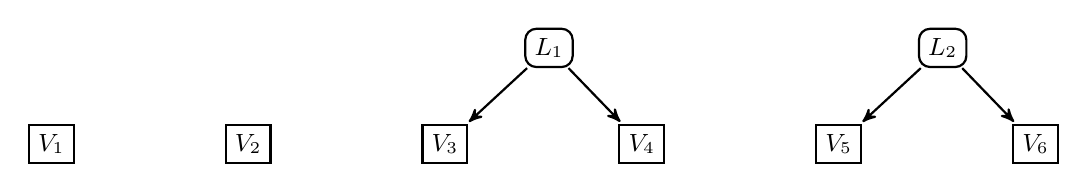
\begin{tikzpicture}[->,>=stealth',shorten >=1pt,auto, node distance=2.5cm,
  thick,main node/.style={rectangle, rounded corners,draw,font=\small\normalfont},
  sq node/.style={rectangle,draw,font=\small\normalfont}]
  \node[sq node] (1) {$V_1$};
  \node[sq node, right of = 1] (2) {$V_2$};
  \node[sq node, right of = 2] (3) {$V_3$};
  \node[sq node, right of = 3] (4) {$V_4$};
  \node[sq node, right of = 4] (5) {$V_5$};
  \node[sq node, right of = 5] (6) {$V_6$};
  \node[main node, above right=1cm of 3] (7) {$L_1$};
  \node[main node, above right=1cm of 5] (8) {$L_2$};
  \path[every node/.style={font=\sffamily\small}]
    (7) edge node  {} (3)
    (7) edge node {} (4)
    (8) edge node {} (5)
    (8) edge node {} (6);
 \end{tikzpicture}
\\
\bigskip
Model 2: \medskip \\
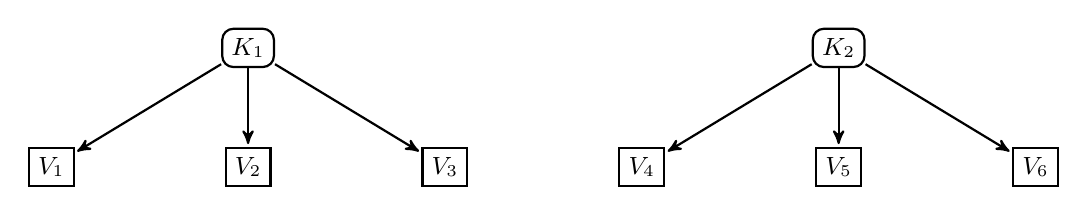
\begin{tikzpicture}[->,>=stealth',shorten >=1pt,auto, node distance=2.5cm,
  thick,main node/.style={rectangle, rounded corners,draw,font=\small\normalfont},
  sq node/.style={rectangle,draw,font=\small\normalfont}]
  \node[sq node] (1) {$V_1$};
  \node[sq node, right of = 1] (2) {$V_2$};
  \node[sq node, right of = 2] (3) {$V_3$};
  \node[sq node, right of = 3] (4) {$V_4$};
  \node[sq node, right of = 4] (5) {$V_5$};
  \node[sq node, right of = 5] (6) {$V_6$};
  \node[main node, above=1cm of 2] (7) {$K_1$};
  \node[main node, above=1cm of 5] (8) {$K_2$};
  \path[every node/.style={font=\small}]
    (7) edge node  {} (1)
    (7) edge node {} (2)
    (7) edge node {} (3)
    (8) edge node {} (4)
    (8) edge node {} (5)
    (8) edge node {} (6);
 \end{tikzpicture}
 \caption{Graphical representations of models used for simulating example data. Square nodes represent observed variables, while rounded nodes represent latent variables. Arrows are used to illustrate causal links.}
\label{fig:simGraphs}
\end{figure}


\begin{figure}[H]
\center
\includegraphics[scale=0.8]{Figure2_v2.pdf}
\caption{CE plots for the simulated datasets. Dataset A (with no differences in data structure) in top panel, and dataset B (where observations stem from different models) in bottom panel. Plots are annotated with the $p$-values of the Kolmogorov-Smirnov (KS) and the Cram\'er-von Mises (CvM) tests of the null hypothesis of no difference in data structures. The bold, black lines illustrate the observed cumulative eigenvalue differences, while the shaded areas are 95 \% confidence bands under the null hypothesis of no difference in data structures.}
\label{plot.simCE} 
\end{figure}

\begin{figure}[H]
\center
\includegraphics[scale=0.8]{Figure3_v2.pdf}
\caption{Angle plots for the simulated datasets. Dataset A in top panel and dataset B in bottom panel. Blue arrows show the principal components of the observations in group 1 decomposed in the coordinate system of the principal components of group 2, while the red arrows illustrate the reverse.}
\label{plot.simAngle}
\end{figure}


\begin{figure}[H]
\center
\includegraphics[scale=0.8]{Figure4_v2.pdf}
\caption{Chroma plots for the simulated datasets. Dataset $\mathbf{A}$ in top panel and dataset $\mathbf{B}$ in bottom panel. Each bar represents a principal component and the bars are annotated with their cumulative percentages of explained variance.}
\label{plot.simChroma}
\end{figure}

\begin{figure}[H]
\center
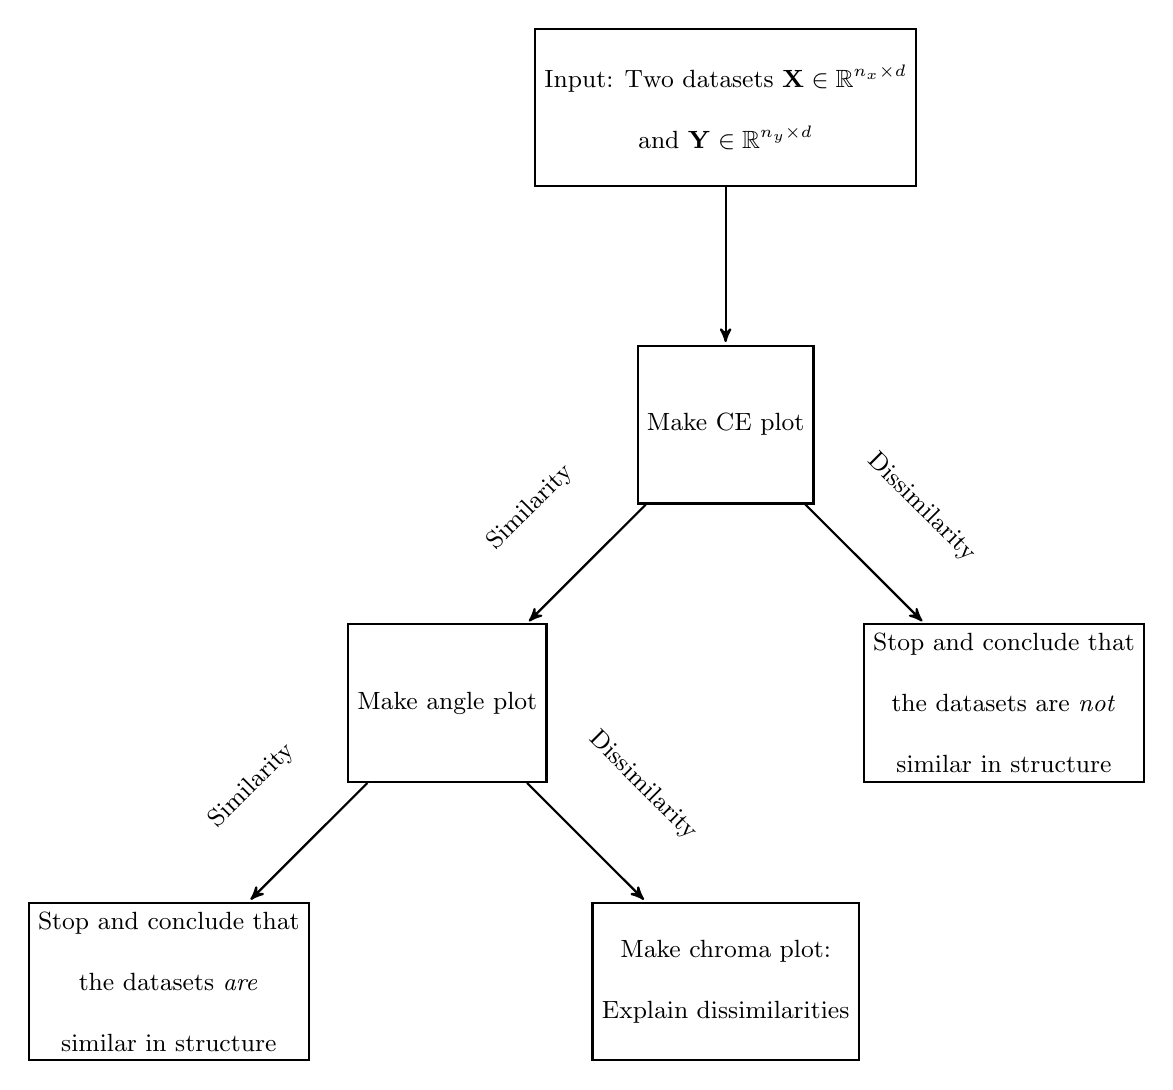
\begin{tikzpicture}[->,>=stealth',shorten >=1pt,auto, node distance=5cm, align=center,
	minimum height=2cm,
  thick,main node/.style={rectangle, rounded corners,draw,font=\small\normalfont},
  sq node/.style={rectangle,draw,font=\small\normalfont}]
  \node[sq node] (1) {Input: Two datasets $\mathbf{X} \in \RR^{n_x \times d}$ \\ and $\mathbf{Y} \in \RR^{n_y \times d}$};
  \node[sq node, below = 2 cm of 1] (2) {Make CE plot};
  \node[sq node, below left of = 2] (3) {Make angle plot};
  \node[sq node, below right of = 2] (4) {Stop and conclude that \\ the datasets are \textit{not} \\ similar in structure};
  \node[sq node, below left of = 3] (5) {Stop and conclude that  \\ the datasets \textit{are} \\ similar in structure};
  \node[sq node, below right of = 3] (6) {Make chroma plot: \\  Explain dissimilarities};
  \path[every node/.style={sloped, anchor = south, font=\small}]
    (1) edge node  {} (2)
    (2) edge node {Similarity} (3)
    (2) edge node {Dissimilarity} (4)
    (3) edge node {Similarity} (5)
    (3) edge node {Dissimilarity} (6);
 \end{tikzpicture}
 \caption{The PCADSC workflow, starting with two datasets and then successively applying the three visual tools for obtaining a deeper and deeper understanding of similarities and dissimilarities in the data structures.}
 \label{fig:flowchart}
 \end{figure}

\begin{figure}[H]
\center
\includegraphics[scale=0.8]{Figure6_v2.pdf}
\caption{CE plots (top panel) and angle plots (bottom panel) comparing Danish and Bulgarian data on psychological well-being. The CE plot is annotated with the $p$-values of the Kolmogorov-Smirnov and the Cram\'er-von Mises tests of the hypothesis of no difference in data structures. In the angle plot, the blue arrows show the principal components of the Bulgarian dataset decomposed in the coordinate system of the principal components of the Danish dataset, while the red arrows illustrate the reverse.}
\label{plotBG.cehair}
\end{figure}

\begin{figure}[H]
\center
\includegraphics[scale=0.8]{Figure7_v2.pdf}
\caption{Chroma plot for comparing Danish and Bulgarian data on psychological well-being. A chroma plot comparing the 2nd, 3rd, and 4th principal components of the Bulgarian- and Danish psychological well-being data. The component-bars are annotated with their relative variance contributions. }
\label{plotBG.pancake}
\end{figure}

\begin{figure}[H]
\center
\includegraphics[scale=0.8]{Figure8_v2.pdf}
\caption{A CE plot (top panel) and an angle plot (bottom panel) comparing Danish and Swedish data on psychological well-being. The blue arrows show the principal components of the Danish dataset decomposed in the coordinate system of the principal components of the Swedish dataset, and the red arrows illustrate the reverse.}
\label{plotSE.cehair}
\end{figure}

\begin{figure}[H]
\center
\includegraphics[scale=0.8]{Figure9_v2.pdf}
\caption{Chroma plot comparing the loading patterns of the Danish and the Swedish subsamples. For each component, the bar is annotated with its cumulative variance contribution, that is, how much variance can be explained by having information of this and the preceding components.}
\label{plotSE.pancake}
\end{figure}

\newpage

\section*{Supplementary material}


\subsection*{S1 Appendix: A brief introduction to principal component analysis}
\label{appendix.introPCA}

In this appendix we introduce PCA. We suppress the subscripts and superscripts used in the article because we only consider a single dataset here, denoted by $\mathbf{X} \in \RR^{d \times n}$. 

For a given $q \leq d$, principal component analysis (PCA) is a tool for finding a new representation of the dataset of dimension $q$ such that the least possible amount of information is lost. More specifically, we wish to minimize the loss when looking at a projection of $\mathbf{X}$ onto a $q$-dimensional space, rather than the original $d$-dimensional one. Formally, we define the \emph{rank-q-reconstruction error} as the minimal squared error that is achievable by linear subspaces $K_q \subset \RR^d$ of dimension $q < d$, that is

\begin{equation}
\min_{K_q} \sum_{i=1}^n \min_{z \in K_q} \lVert x_{i \cdot} - \bar{X} - z \rVert^2 =
\min_{K_q} \sum_{i=1}^n \lVert x_{i \cdot} - \bar{X} - \text{proj}_{K_q}(x_{i \cdot} - \bar{X}) \rVert^2.
\end{equation}

The theory of \emph{Principal component analysis} (PCA) not only ensures the existence of a subspace $\hat{K}_q \subset \RR^d$ that attains this minimum, it also provides an explicit description of $\hat{K}_q$ and the rank-q-reconstruction error \cite{HastieEtAl2009}. More specifically, the rank-q-reconstruction error is attained when we choose

\begin{equation*}
\hat{K}_q = \text{span}\{\eta_1,\dotsc,\eta_q\},
\end{equation*}
where $\eta_1, ..., \eta_q$ are the first $q$ eigenvectors of the empirical covariance matrix, $S$, as ordered by the size of their associated eigenvalues, $\lambda_1, \dotsc, \lambda_d$. In the PCA framework, we refer to the eigenvectors as \textit{loadings}. The eigenvalues may be understood as \textit{variance components}, as the sum of the marginal empirical variances is preserved under eigenvalue decomposition, that is,
\begin{equation*}
\text{trace}(S) = \sum_{j=1}^d \hat{V}(X_j) = \sum_{j=1}^d \hat{V}(\eta_j^\top \mathbf{X}^\top) = \sum_{j=1}^d \lambda_j,
\end{equation*}
where $X_j \in \RR^n$ denotes the $j$th variable of $\mathbf{X}$ and $\hat{V}$ is the empirical variance function. This again emphasizes that we do not change the covariance structure of a dataset when performing PCA; we merely use linear algebra to make it easier to describe. And as eigenvalues are uniquely defined, and eigenvectors are uniquely defined up to a change of sign whenever the eigenvalues are distinct, the representation hereby obtained is a valid object of inference. 

The $j$th loading can also be found iteratively as the unit vector $u \in \RR^d$ orthogonal to $\hat{K}_{j-1}$ that maximizes the variation of the associated scores:
\begin{align*}
\eta_j &= \argmax_{u \in \RR^d\colon u \perp \hat{K}_{j-1}} \sum_{i=1}^n \lVert u^\top (x_{i \cdot} - \bar{X}) \rVert^2, &
\lambda_j &= \frac{1}{n-1} \sum_{i=1}^n \lVert \eta_j^\top (x_{i \cdot} - \bar{X}) \rVert^2,
\end{align*}
where the initial subspace is defined as $\hat{K}_0 = \{0\}$. It is worth emphasizing that this greedy approach of successively adding the next direction $\eta_j$ explaining most of the remaining variation also gives the sequence $\hat{K}_q = \hat{K}_{q-1} \oplus \text{span} \{\eta_q\}$ of subspaces minimizing the rank-q-reconstruction error.

At this point a general remark about standardization is in place. PCA deconstructs the covariance matrix in components according to the most explained variance. This implies that if a variable has a very large sample variance (possibly because of its scale), this variable will always be deemed highly influential, no matter the structure of the data. Therefore, the variables are typically standardized prior to performing PCA. The covariance matrix of the standardized variables is the same as the correlation matrix of the original variables, so post-standardization PCA simply corresponds to performing data structure comparisons of the correlation matrices rather than the covariance matrices. The standardization makes the variables comparable on the same scale, namely units of standard deviation. We have adopted this standardization policy. 



\subsection*{S2 Appendix: Details about the simulated data}
\label{appendix.simData}
This supplementary appendix describes the origin of the simulated data used for presenting the PCADSC plots. Dataset $\mathbf{A}$ consisted of 1000 independent simulated realizations from the $N(0, \Sigma_1)$-distribution, while dataset $\mathbf{B}$ consisted of 500 independent realizations from $N(0, \Sigma_1)$ and 500 independent realizations from $N(0, \Sigma_2)$. Dataset $\mathbf{A}$ was furthermore appended with a grouping variable, randomly dividing the observations into two groups. Dataset $\mathbf{B}$ also included a grouping variable, and this variable contained information about which of the two normal distributions each observation was simulated from. The covariance matrices, $\Sigma_A$ and $\Sigma_B$, were defined by

$$\Sigma_A = \begin{pmatrix}
    1.0  &  0.0 & 0.0 & 0.0 & 0.0 & 0.0 \\
 0.0  &  1.0 & 0.0 & 0.0&  0.0 & 0.0 \\
 0.0   & 0.0 &  1.0 & 0.7 & 0.0 & 0.0 \\
 0.0 &  0.0 & 0.7 & 1.0 & 0.0 & 0.0 \\
0.0 &    0.0 &  0.0 & 0.0 & 1.0 & 0.4 \\
 0.0 & 0.0 &  0.0 & 0.0 & 0.4 & 1.0
\end{pmatrix}$$
and
$$
\Sigma_B = \begin{pmatrix}
 1.0 & 0.2 & 0.1 & 0.0 & 0.0 & 0.0 \\
 0.2 & 1.0 & 0.1 & 0.0 & 0.0 & 0.0 \\
 0.1 & 0.1 & 1.0 & 0.0 & 0.0 & 0.0 \\
 0.0 & 0.0 & 0.0 & 1.0 & 0.3 & 0.1 \\
 0.0 & 0.0 & 0.0 & 0.3 & 1.0 & 0.2 \\
 0.0 & 0.0 & 0.0 & 0.1 & 0.2 & 1.0
\end{pmatrix},
$$
respectively.


\subsection*{S3 Table: ESS psychological wellbeing scale definitions}
\begin{table}[h]
\centering
\caption{{\bf ESS psychological wellbeing scale definitions.} Relationship between questionnaire items and scales, as defined in \cite{ESStopline5}. Before we construct the scale scores as item means, we transform the individual item scores such that they are all on a scale from 0 to 10 and such that 10 always corresponds being the most happy.}
\label{table:items}

\scriptsize
\rowcolors{1}{}{lightgray}
\bgroup
\def\arraystretch{1.5}
\begin{tabular}{ll}
\hline
Scale & Items \\
\hline
\rowcolor{lightgray} & How satisfied with life as a whole \\
\rowcolor{lightgray}\multirow{-2}{*}{Evaluative wellbeing }& How happy are you\\

\rowcolor{white} & Felt sad, how often in the past week\\
\rowcolor{white} & Felt depressed, how often in the past week\\
\rowcolor{white} & Enjoyed life, how often in the past week\\
\rowcolor{white} & Were happy, how often in the past week\\
\rowcolor{white} & Felt anxious, how often in the past week\\
\rowcolor{white}\multirow{-6}{*}{Emotional wellbeing} & Felt calm and peaceful, how often in the past week\\

\rowcolor{lightgray} & Free to decide how to live my life\\
\rowcolor{lightgray} & Little chance to show how capable I am\\
\rowcolor{lightgray} & Feel accomplishment from what I do\\
\rowcolor{lightgray} & Interested in what you are doing\\
\rowcolor{lightgray} & Absorbed in what you are doing\\
\rowcolor{lightgray} & Enthusiastic about what you are doing\\
\rowcolor{lightgray} & Feel what I do in life is valuable and worthwhile\\
\rowcolor{lightgray} & Have a sense of direction\\
\rowcolor{lightgray} & Always optimistic about my future\\
\rowcolor{lightgray} & There are lots of things I feel I am good at\\
\rowcolor{lightgray} & In general feel very positive about myself\\
\rowcolor{lightgray} & At times feel as if I am a failure\\
\rowcolor{lightgray} & When things go wrong in my life it takes a long time to get back to normal\\
\rowcolor{lightgray}\multirow{-14}{*}{Functioning} & Deal with important problems\\

\rowcolor{white} & Felt everything did as effort, how often in the past week\\
\rowcolor{white} & Sleep was restless, how often in the past week\\
\rowcolor{white} & Could not get going, how often in the past week\\
\rowcolor{white}\multirow{-4}{*}{Vitality} & Had a lot of energy, how often in the past week\\

\rowcolor{lightgray} &  Most people can be trusted\\
\rowcolor{lightgray} &  People try to take advantage\\
\rowcolor{lightgray} &  Most of the time people are helpful\\
\rowcolor{lightgray} &  Feel people in local area help one another\\
\rowcolor{lightgray}\multirow{-5}{*}{Community wellbeing}& Feel close to the people in local area\\

\rowcolor{white} & How many with whom you can discuss intimate matters\\
\rowcolor{white} & Feel appreciated by those you are close to\\
\rowcolor{white} & Receive help and support\\
\rowcolor{white}\multirow{-4}{*}{Supportive relationships} & Felt lonely, how often in the past week\\
\hline
\end{tabular}
\egroup
\end{table}
\end{document}




